%\documentclass[aps,pra,amsmath,amssymb,floatfix,twocolumn, amsmath, superscriptaddress, twocolumn]{revtex4}
\documentclass[aps,amsmath,prl]{revtex4-2}
\usepackage{multirow}
\usepackage{bbold}
\usepackage{subfigure}
\usepackage{color}
\usepackage{mathrsfs}
%\usepackage{hyperref}

\newcommand{\pg}[1]{\textcolor{red}{#1}}
\newcommand{\bvec}[1]{{\mathbf #1}}
%\newcommand{\bra}[1]{\left< #1 \right|}
%\newcommand{\ket}[1]{\left| #1 \right>}


\usepackage{amsfonts, relsize, color}
\usepackage{graphics}
\usepackage{graphicx}
\usepackage{subfigure}
\usepackage{hyperref}
\usepackage{color}
\usepackage{physics}
\newcommand{\expect}[1]{#1}
\renewcommand\vec[1]{\ensuremath\boldsymbol{#1}} % bold font for vectors

%\usepackage[english]{babel}
\usepackage[utf8]{inputenc}
\usepackage{fancyhdr}

\pagestyle{fancy}
\fancyhf{}
\rhead{Effects of Berry Curvature on Thermoelectric Transport ...}
\lhead{A. Panigrahi}
\rfoot{Page \thepage}



\begin{document}


\title{\bf Effects of Berry Curvature on Thermoelectric Transport of Bilayer Graphene and Other Materials}


\author{Archisman Panigrahi}
\affiliation{Indian Institute of Science, Bangalore 560012, India}



\date{\today}

\begin{abstract}

\end{abstract}

\maketitle

\onecolumngrid


%%%%%%%%%%%%%%%%%%%%%%%%%%%%%%%%%%%%%%%%%%%%%%%%%%%%%%
%%%%%%%%%%%%%%%%%%%%%%%%%%%%%%%%%%%%%%%%%%%%%%%%%%%%%%
%%%%%%%%%%%%%%%%%%%%%%%%%%%%%%%%%%%%%%%%%%%%%%%%%%%%%%
%%%%%%%%%%%%%%%%%%%%%%%%%%%%%%%%%%%%%%%%%%%%%%%%%%%%%%
%%%%%%%%%%%%%%%%%%%%%%%%%%%%%%%%%%%%%%%%%%%%%%%%%%%%%%

\section{Introduction}
intro
\section{Berry curvature in reciprocal space}
\subsection{Berry Curvature}
When the Hamiltonian of a system has a paramater $\vec{\lambda}$ which evolves slowly (compared to the timescale $\frac{\hbar}{\varepsilon}$ of a state $\ket{\varepsilon}$), an eigenstate of the Hamiltonian evolves as,\cite{BerryQuantalPhase1984}

\begin{equation}
	\ket{\varepsilon(\vec{\lambda}(t))} = e^{i \gamma(t)} e^{-\frac{i}{\hbar} \int_0^t \varepsilon(\vec{\lambda}(t')) dt'} \ket{\varepsilon(\vec{\lambda}(0))}
\end{equation}
where the geometric phase $\gamma(t)$ is given by $i\int_{\vec{\lambda}_i}^{\vec{\lambda}_f} \bra{\varepsilon({\vec{\lambda}})}\nabla_{\vec{\lambda}} \ket{\varepsilon({\vec{\lambda}})} \cdot d \vec{\lambda}$. It depends on the trajectory in the parameter space $\vec{\lambda}$, not just the endpoints. The real quantity $i\bra{\varepsilon({\vec{\lambda}})}\nabla_{\vec{\lambda}}\ket{\varepsilon({\vec{\lambda}})} = \vec{A(\vec{\lambda})}$ is known as the Berry connection, and its curl, $\vec{\Omega} = \nabla_{\vec{\lambda}} \times \vec{A}$ is known as the Berry curvature.

\textbf{Note}: $\bra{\varepsilon({\vec{\lambda}})}\nabla_{\vec{\lambda}} \ket{\varepsilon({\vec{\lambda}})}$ stands for $\int d\vec{r} \varepsilon_{\vec{\lambda}}^* (\vec{r}) \nabla_{\vec{\lambda}} \varepsilon_{\vec{\lambda}}(\vec{r})$, where $\varepsilon_{\vec{\lambda}}(\vec{r})$ is the normalized position space wavefunction of $\ket{\varepsilon({\vec{\lambda}})}$.

While the overall phase of the state does not affect its physical observables, if we take a linear combination of such eigenstates, each of them would evolve with a different geometric phase, and that would indeed affect the physical properties of the system. We would now see how such a geometric phase manifests in electrons moving in a lattice, when an external electromagnetic field is applied.

\subsection{Electrons in a lattice}
Now, let us consider an electron in a periodic potential $V(\vec{r})$ (e.g. the potential due to a lattice), without any external fields. The Hamiltonian describing it is given by $\hat{H} = \frac{{\hat{\vec{p}}}^2}{2 m} + V(\hat{\vec{r}})$.

The eigenfunctions of this Hamiltonian are of the form,
$$\psi_{n, \vec{k}} (\vec{r}) = e^{i \vec{k}\cdot \vec{r}} u_{n,\vec{k}} (\vec{r})$$

Here $u_{n,\vec{k}} (\vec{r})$ is a function with the same periodicity as $V(\vec{r})$ (e.g. in a lattice, it would be periodic in every unit cell). The quantity $\hbar \bvec{k}$ is known as the crystal momentum and $n$ is the band index. This result is known as Bloch's theorem (See chapter 8 of \cite{AshcroftMermin76}). The crystal momentum is a good quantum number for an electron in a lattice, and it is conserved upto a reciprocal lattice vector (times $\hbar$).
Now, we can rewrite the eigenvalue equation $\hat{H} \psi_{n, \vec{k}}(\vec{r}) = \varepsilon_{n,\vec{k}} \psi_{n, \vec{k}}(\vec{r})$ as,
\begin{equation}~\label{Eq:effectiveBlochEquation}
	\left[\frac{\hbar^2}{2m}(\vec{k} - i \nabla)^2 + V(\vec{r}) \right]u_{n,\vec{k}} (\vec{r}) = \varepsilon_{n,\vec{k}} u_{n,\vec{k}} (\vec{r})
\end{equation}

In this equation, $\vec{k}$ is just a parameter in the effective Hamiltonian. When we apply an external electromagnetic field, the crystal momentum is not anymore a good quantum number. Its evolution is governed by the Lorenz force, (See Appendix \ref{app:crystal-momentum-time-evolution})

\begin{equation} \label{Eq:evolution-of-k}
	\hbar \dot{\vec{k}} = -e\left(\vec{E} + \langle\dot{\vec{r}}\rangle \times \vec{B} \right)
\end{equation}

As $\vec{k}$ changes, it would give rise to a geometric phase. After a small time interval $\Delta t$, $\vec{k}$ would evolve to $\vec{k} + \Delta \vec{k}$ (with $\Delta \vec{k} = \dot{\vec{k}} \Delta t$), and the wavefunction of a state labeled with $\vec{k}$ would evolve as $u_{n, \vec{k}} \rightarrow e^{i \vec{A}\cdot \vec{\Delta{k}}} e^{-i \frac{\varepsilon_{\vec{k}} \Delta t}{\hbar}} u_{n, \vec{k}+\Delta \vec{k}}$, where $\vec{A}(\vec{k})=i \bra{u_{n,\vec{k}}}\nabla_{\vec{k}} \ket{u_{n,\vec{k}}}$ is the Berry connection in the reciprocal space. Again, for a state labeled with a single $\vec{k}$, this geometric phase is an overall global phase, which would not show up in physical observables. However, if we take a linear superposition of Bloch wavefunctions with different values of $\vec{k}$, each of them would evolve with a different geometric phase $\gamma_n (\vec{k}) = \int_{0}^{t} dt' \vec{A(\vec{k})} \cdot \frac{d \vec{k}}{dt'} $, and we would soon see that the interference of such phase factors would lead to many interesting effects.
\section{Effects of Berry Curvature}
\subsection{Modification of semiclassical equations of motion of an wavepacket}
The probability density of the wavefunction $\psi_{n, \vec{k}} (\vec{r}) = e^{i \vec{k}\cdot \vec{r}} u_{n,\vec{k}} (\vec{r})$ is not localized anywhere, it is periodic over all unit cells (The blue curve in Fig. \ref{fig:wavepacket-and-bloch-wave}). We can construct a wave packet by forming a linear superposition of many such states, such that the wavepacket is localized at some point $\vec{r}_0$ in the real space, and its crystal momentum is also localized around a value of $\hbar \vec{k}_0$.
\begin{figure}
	\centering
	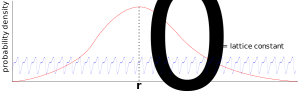
\includegraphics[width=0.7\linewidth]{wavepacket-and-Bloch-wave}
	\caption{The red}
	\label{fig:wavepacket-and-bloch-wave}
\end{figure}


\subsection{Violation of Liouville's theorem and Modification of phase space density}
Derivation from the semiclassical equations of Motion
\section{Decoupling of the equations of motion and their simplification}
\begin{equation}~\label{Eq:SC_EOM_r_dot}
	\dot{\bvec{r}} = \frac{\frac{1}{\hbar} \frac{\partial \varepsilon}{\partial \bvec{k}} + \frac{e}{\hbar} (\bvec{E}\times\bvec{\Omega}) + \frac{e}{\hbar^2} (\Omega \cdot \frac{\partial \varepsilon}{\partial \bvec{k}} )\bvec{B}}{1 + \frac{e}{\hbar} \bvec{B}\cdot\bvec{\Omega}}
\end{equation}

\begin{equation}~\label{Eq:SC_EOM_k_dot}
	\dot{\bvec{k}} = -\frac{\frac{e}{\hbar} \bvec{E} +\frac{e}{\hbar^2} \frac{\partial \varepsilon}{\partial \bvec{k}} \times \bvec{B} + \frac{e^2}{\hbar^2} (\bvec{E}\cdot\bvec{B})\Omega}{1 + \frac{e}{\hbar} \bvec{B}\cdot\bvec{\Omega}}
\end{equation}
In a 2D sample, $\bvec{\Omega}$ is along the $z$ axis, while $\frac{\partial \varepsilon}{\partial \bvec{k}}$ is in the $xy$ plane, then $\bvec{\Omega} \cdot \frac{\partial \varepsilon}{\partial \bvec{k}} = 0$.

Also, if we take perpendicular electric and magnetic fields, then $\bvec{E}\cdot \bvec{B} = 0$.

Then the equations \eqref{Eq:SC_EOM_r_dot} and \eqref{Eq:SC_EOM_k_dot} simplify to,
\begin{equation}~\label{Eq:SC_EOM_r_dot_decoupled}
	\dot{\bvec{r}} = \frac{\frac{1}{\hbar} \frac{\partial \varepsilon}{\partial \bvec{k}} + \frac{e}{\hbar} (\bvec{E}\times\bvec{\Omega})}{1 + \frac{e}{\hbar} \bvec{B}\cdot\bvec{\Omega}}
\end{equation}

\begin{equation}~\label{Eq:SC_EOM_k_dot_decoupled}
	\dot{\bvec{k}} = -\frac{\frac{e}{\hbar} \bvec{E} +\frac{e}{\hbar^2} \frac{\partial \varepsilon}{\partial \bvec{k}} \times \bvec{B}}{1 + \frac{e}{\hbar} \bvec{B}\cdot\bvec{\Omega}}
\end{equation}
\section{Strategy of Calculation of Thermal and Heat Currents}
\subsection{Equilibrium and Non-Equilibrium distribution functions}
\section{Boltzmann Transport Equation and its solution}
Some discussions about the relaxation time approximation....

Under the relaxation time approximation, the Boltzmann Transport Equation (BTE) takes the form
\begin{equation}~\label{Eq:BTE}
\dot{\bvec{k}}\cdot\frac{\partial}{\partial \bvec{k}} (f + g) + \dot{\bvec{r}}\cdot\frac{\partial}{\partial \bvec{r}} (f + g) = -\frac{g}{\tau}
\end{equation},

which can be cast into the form
\begin{equation}~\label{Eq:BTE2}
	\frac{g}{\tau} + \dot{\bvec{k}}\cdot\frac{\partial}{\partial \bvec{k}} g + \dot{\bvec{r}}\cdot\frac{\partial}{\partial \bvec{r}} g = -\dot{\bvec{k}}\cdot\frac{\partial}{\partial \bvec{k}}f - \dot{\bvec{r}}\cdot\frac{\partial}{\partial \bvec{r}}f
\end{equation}.

Here $f = \frac{1}{e^{\beta(\varepsilon_{\bvec{k}} - \mu)} + 1}$ is the equilibrium Fermi distribution, and $g$ is the non-equilibrium part.
Using the decoupled equations of motion, right hand side of Eq. \eqref{Eq:BTE2} simplifies to (\textit{Need to show the steps}),
$$\frac{\partial f}{\partial \varepsilon}\frac{1}{1 + \frac{e}{\hbar} \bvec{B}\cdot\bvec{\Omega}}
\frac{1}{\hbar} \frac{\partial \varepsilon}{\partial \bvec{k}}\cdot\left[e \bvec{E} + \nabla{\mu} + \nabla T \frac{\varepsilon - \mu}{T}\right]
$$.

When the fields are constant in space and time, we assume that $\frac{\partial{g}}{\partial \bvec{r}} = 0$.

\textbf{Validity of the assumption}: When we solve the equation after discarding this term, we would find that (See Eq. ~\eqref{Eq:gnonzeroE}) this term is second order in the applied fields. Then upto linear order, we can discard this term.

Then, the BTE becomes,
$\frac{g}{\tau} -\frac{\frac{e}{\hbar} \bvec{E} +\frac{e}{\hbar^2} \frac{\partial \varepsilon}{\partial \bvec{k}} \times \bvec{B}}{1 + \frac{e}{\hbar} \bvec{B}\cdot\bvec{\Omega}} \cdot\frac{\partial}{\partial \bvec{k}} g = \frac{\partial f}{\partial \varepsilon}\frac{1}{1 + \frac{e}{\hbar} \bvec{B}\cdot\bvec{\Omega}}
\frac{1}{\hbar} \frac{\partial \varepsilon}{\partial \bvec{k}}\cdot\left[e \bvec{E} + \nabla{\mu} + \nabla T \frac{\varepsilon - \mu}{T}\right] $

%\subsection{Solution at $\bvec{B}=0$, $\bvec{\Omega}=0$}
%\subsection{Solution at $\bvec{B}\neq0$, $\bvec{\Omega}=0$}
%\subsection{Solution at $\bvec{B}\neq0$, $\bvec{\Omega}\neq 0$, $\bvec{E} \neq 0$, $\bvec{\mu}

\subsection{Solution for $\bvec{B}\neq0$, $\bvec{\Omega}\neq 0$, $\bvec{E} \neq 0$, $\nabla \mu = \nabla T = 0$}

In this limit, the equation becomes,
$$
\frac{g}{\tau} -\frac{\frac{e}{\hbar} \bvec{E} +\frac{e}{\hbar^2} \frac{\partial \varepsilon}{\partial \bvec{k}} \times \bvec{B}}{1 + \frac{e}{\hbar} \bvec{B}\cdot\bvec{\Omega}} \cdot\frac{\partial}{\partial \bvec{k}} g = \frac{\partial f}{\partial \varepsilon}\frac{1}{1 + \frac{e}{\hbar} \bvec{B}\cdot\bvec{\Omega}}
\frac{1}{\hbar} \frac{\partial \varepsilon}{\partial \bvec{k}}\cdot e \bvec{E} $$

If we discard the term $\bvec{E} \cdot \frac{\partial \varepsilon}{\partial \bvec{k}}$ in the LHS, we would find that $g$ is a linear function of $\bvec{E}$. Then, $\bvec{E} \cdot \frac{\partial \varepsilon}{\partial \bvec{k}}$ would be quadratic in $\bvec{E}$. This is why, we can discard this term. (This is not a circular argument. If we do this, everything remains self consistent upto linear order)

Then, the equation takes the form,
\begin{equation}
\frac{g}{\tau} -\frac{\frac{e}{\hbar^2} }{1 + \frac{e}{\hbar} \bvec{B}\cdot\bvec{\Omega}} \frac{\partial \varepsilon}{\partial \bvec{k}} \times \bvec{B} \cdot\frac{\partial}{\partial \bvec{k}} g = \frac{\partial f}{\partial \varepsilon}\frac{1}{1 + \frac{e}{\hbar} \bvec{B}\cdot\bvec{\Omega}}
\frac{1}{\hbar} \frac{\partial \varepsilon}{\partial \bvec{k}}\cdot e \bvec{E}
\end{equation}~\label{Eq:BTE_zero_chem_pot_thermal_gradient}

We solve this equation, treating the second term in LHS as a perturbation (See Appendix \ref{app:perturbation_validation}).
We write $g = g_0 + g_1$, such that $\frac{g_0}{\tau} = \frac{\partial f}{\partial \varepsilon}\frac{1}{1 + \frac{e}{\hbar} \bvec{B}\cdot\bvec{\Omega}}
\frac{1}{\hbar} \frac{\partial \varepsilon}{\partial \bvec{k}}\cdot e \bvec{E}$, and $\frac{g_1}{\tau} -\frac{\frac{e}{\hbar^2} }{1 + \frac{e}{\hbar} \bvec{B}\cdot\bvec{\Omega}} \frac{\partial \varepsilon}{\partial \bvec{k}} \times \bvec{B} \cdot\frac{\partial}{\partial \bvec{k}} g_0 = 0$.
Then, $g_1$ is a linear function of $\bvec{B}$, and it is justified to discard the term $\frac{\frac{e}{\hbar^2} }{1 + \frac{e}{\hbar} \bvec{B}\cdot\bvec{\Omega}} \frac{\partial \varepsilon}{\partial \bvec{k}} \times \bvec{B} \cdot\frac{\partial}{\partial \bvec{k}} g_1$, as it would be quadratic in $\bvec{B}$


Then, ${g_0} = \frac{\partial f} {\partial \varepsilon}\frac{1}{1 + \frac{e}{\hbar} \bvec{B}\cdot\bvec{\Omega}}
\frac{e \tau}{\hbar} \frac{\partial \varepsilon}{\partial \bvec{k}}\cdot \bvec{E}$. To find $g_1$, we need to calculate $\frac{\partial g_0}{\partial \bvec{k}}$, i.e., the quantity 
$\frac{\partial}{\partial \bvec{k}} \left[ \frac{\partial f} {\partial \varepsilon}\frac{1}{1 + \frac{e}{\hbar} \bvec{B}\cdot\bvec{\Omega}}
\frac{e \tau}{\hbar} \frac{\partial \varepsilon}{\partial \bvec{k}}\cdot \bvec{E} \right]$.

To calculate it, let us first calculate $\nabla \left[\phi \bvec{A}\cdot\bvec{C}\right]$, where $\phi$ is a scalar function, $\bvec{A}$ is a vector function, and $\bvec{C}$ is a constant vector.

$\nabla \left[\phi \bvec{A}\cdot\bvec{C}\right] = (\nabla \phi) (\bvec{A}\cdot\bvec{C}) + \phi (\bvec{C}\cdot \nabla){A} + \phi (\bvec{C}\times(\nabla\times\bvec{A})) $. In our calculation, $\phi \sim \frac{\partial f} {\partial \varepsilon}\frac{1}{1 + \frac{e}{\hbar} \bvec{B}\cdot\bvec{\Omega}}
\frac{e \tau}{\hbar}$, $\bvec{A} \sim \frac{\partial \varepsilon}{\partial \bvec{k}}$, and $\bvec{C} \sim \bvec{E}$.

Then, $$\frac{\partial}{\partial \bvec{k}} \left[ \frac{\partial f} {\partial \varepsilon}\frac{1}{1 + \frac{e}{\hbar} \bvec{B}\cdot\bvec{\Omega}}
\frac{e \tau}{\hbar} \frac{\partial \varepsilon}{\partial \bvec{k}}\cdot \bvec{E} \right] = \frac{\partial}{\partial \bvec{k}} \left[ \frac{\frac{\partial f} {\partial \varepsilon} \tau}{1 + \frac{e}{\hbar} \bvec{B}\cdot\bvec{\Omega}}
 \right] \frac{e \bvec{E}}{\hbar} \cdot \frac{\partial \varepsilon}{\partial \bvec{k}} + \frac{\frac{\partial f} {\partial \varepsilon} \tau}{1 + \frac{e}{\hbar} \bvec{B}\cdot\bvec{\Omega}} \left[(\frac{e}{\hbar} \bvec{E}\cdot \frac{\partial }{\partial \bvec{k}} )\frac{\partial \varepsilon}{\partial \bvec{k}} + \frac{e}{\hbar} \bvec{E}\times (\frac{\partial }{\partial \bvec{k}} \times \frac{\partial \varepsilon}{\partial \bvec{k}}) \right]$$.
 
 The last term is zero because it is the curl of a gradient, $\frac{\partial }{\partial \bvec{k}} \times \frac{\partial \varepsilon}{\partial \bvec{k}} = \nabla_\bvec{k} \times (\nabla_\bvec{k} \varepsilon) = 0$.
 
 Finally,
\begin{equation}\label{Eq:gnonzeroE}
 g = \frac{\partial f} {\partial \varepsilon}\frac{1}{1 + \frac{e}{\hbar} \bvec{B}\cdot\bvec{\Omega}}
 \frac{\tau}{\hbar} \frac{\partial \varepsilon}{\partial \bvec{k}}\cdot e \bvec{E} + \frac{\frac{e \tau}{\hbar^2} }{1 + \frac{e}{\hbar} \bvec{B}\cdot\bvec{\Omega}} \frac{\partial \varepsilon}{\partial \bvec{k}} \cdot \bvec{B} \times \left[ \frac{\partial}{\partial \bvec{k}} \left[ \frac{\frac{\partial f} {\partial \varepsilon} \tau}{1 + \frac{e}{\hbar} \bvec{B}\cdot\bvec{\Omega}}
 \right] \frac{e \bvec{E}}{\hbar} \cdot \frac{\partial \varepsilon}{\partial \bvec{k}} + \frac{\frac{\partial f} {\partial \varepsilon} \tau}{1 + \frac{e}{\hbar} \bvec{B}\cdot\bvec{\Omega}} \left[(\frac{e}{\hbar} \bvec{E}\cdot \frac{\partial }{\partial \bvec{k}} )\frac{\partial \varepsilon}{\partial \bvec{k}} \right] \right]
 \end{equation}
 
Verification: When $\vec{\Omega} = 0$, and $\varepsilon = \frac{\hbar^2 k^2}{2 m^*}$, this term produces $\sigma_{xy} = -\omega_c \tau \frac{n e^2 \tau}{m^*}$.
(\textit{Need to show the steps})

\subsection{Solution for $\bvec{B}\neq0$, $\bvec{\Omega}\neq 0$, $\bvec{E} = 0$, $\nabla \mu \neq 0$, $\nabla T \neq 0$}

Here \begin{equation}
\dot{\bvec{r}} = \frac{\frac{1}{\hbar} \frac{\partial \varepsilon}{\partial \bvec{k}}}{1 + \frac{e}{\hbar} \bvec{B}\cdot\bvec{\Omega}}
\end{equation}

\begin{equation}
\dot{\bvec{k}} = -\frac{\frac{e}{\hbar^2} \frac{\partial \varepsilon}{\partial \bvec{k}} \times \bvec{B}}{1 + \frac{e}{\hbar} \bvec{B}\cdot\bvec{\Omega}}
\end{equation}

We again take $\frac{\partial g}{\partial \bvec{k}} \sim 0$.

Under these circumstances, the equation becomes,
$$
\frac{g}{\tau} -\frac{\frac{e}{\hbar^2} \frac{\partial \varepsilon}{\partial \bvec{k}} \times \bvec{B}}{1 + \frac{e}{\hbar} \bvec{B}\cdot\bvec{\Omega}} \cdot\frac{\partial}{\partial \bvec{k}} g = \frac{\partial f}{\partial \varepsilon}\frac{1}{1 + \frac{e}{\hbar} \bvec{B}\cdot\bvec{\Omega}}
\frac{1}{\hbar} \frac{\partial \varepsilon}{\partial \bvec{k}}\cdot\left[ \nabla{\mu} + \nabla T \frac{\varepsilon - \mu}{T}\right] $$

Let $g = g_0 + g_1$, with $g_0 = \frac{\partial f}{\partial \varepsilon}\frac{1}{1 + \frac{e}{\hbar} \bvec{B}\cdot\bvec{\Omega}}
\frac{\tau}{\hbar} \frac{\partial \varepsilon}{\partial \bvec{k}}\cdot\left[ \nabla{\mu} + \nabla T \frac{\varepsilon - \mu}{T}\right]$ and $\frac{g_1}{\tau} -\frac{\frac{e}{\hbar^2} \frac{\partial \varepsilon}{\partial \bvec{k}} \times \bvec{B}}{1 + \frac{e}{\hbar} \bvec{B}\cdot\bvec{\Omega}} \cdot\frac{\partial}{\partial \bvec{k}} g_0 = 0$

Then, \textit{(Need to show the steps)}
$$\frac{\partial g_0}{\partial \bvec{k}} = 
\frac{\partial}{\partial \bvec{k}} \left[ \frac{\frac{\partial f} {\partial \varepsilon} \tau}{1 + \frac{e}{\hbar} \bvec{B}\cdot\bvec{\Omega}}
\right] \frac{\nabla \mu + \frac{\varepsilon - \mu}{T}}{\hbar} \cdot \frac{\partial \varepsilon}{\partial \bvec{k}} + \frac{\frac{\partial f} {\partial \varepsilon} \tau}{1 + \frac{e}{\hbar} \bvec{B}\cdot\bvec{\Omega}} \left[(\frac{\nabla \mu + \frac{\varepsilon - \mu}{T}}{\hbar} \cdot \frac{\partial }{\partial \bvec{k}} )\frac{\partial \varepsilon}{\partial \bvec{k}} + \frac{1}{\hbar} (\nabla \mu + \frac{\varepsilon - \mu}{T})\times \underbrace{(\frac{\partial }{\partial \bvec{k}} \times \frac{\partial \varepsilon}{\partial \bvec{k}})}_0 \right]
$$
$$+ \frac{\frac{\partial f} {\partial \varepsilon} \tau}{1 + \frac{e}{\hbar} \bvec{B}\cdot\bvec{\Omega}} \left[\frac{1}{\hbar} (\frac{\partial \varepsilon}{\partial \bvec{k}} \cdot \frac{\partial }{\partial \bvec{k}}) (\frac{\varepsilon \nabla T}{T}) + \frac{1}{\hbar} \frac{\partial \varepsilon}{\partial \bvec{k}} \times \left(  \frac{\partial }{\partial \bvec{k}} \times \left(\frac{\varepsilon \nabla T}{T}\right) \right) \right]$$

The term inside the final third bracket can be further simplified.

$$ (\frac{\partial \varepsilon}{\partial \bvec{k}} \cdot \frac{\partial }{\partial \bvec{k}}) (\frac{\varepsilon \nabla T}{T}) + \frac{\partial \varepsilon}{\partial \bvec{k}} \times \left(  \frac{\partial }{\partial \bvec{k}} \times \left(\frac{\varepsilon \nabla T}{T}\right) \right) = (\frac{\partial \varepsilon}{\partial \bvec{k}} \cdot \frac{\partial \varepsilon}{\partial \bvec{k}}) (\frac{ \nabla T}{T}) + \frac{\partial \varepsilon}{\partial \bvec{k}} \times \left(  \frac{\partial \varepsilon}{\partial \bvec{k}} \times \left(\frac{\nabla T}{T}\right) \right)$$
$$  =(\frac{\partial \varepsilon}{\partial \bvec{k}} \cdot \frac{\partial \varepsilon}{\partial \bvec{k}}) (\frac{ \nabla T}{T}) + \left(  \frac{\partial \varepsilon}{\partial \bvec{k}} \cdot \frac{\nabla T}{T}\right) \frac{\partial \varepsilon}{\partial \bvec{k}} -  (\frac{\partial \varepsilon}{\partial \bvec{k}} \cdot \frac{\partial \varepsilon}{\partial \bvec{k}}) (\frac{ \nabla T}{T})$$
$$= \left(  \frac{\partial \varepsilon}{\partial \bvec{k}} \cdot \frac{\nabla T}{T}\right) \frac{\partial \varepsilon}{\partial \bvec{k}}$$.

When we calculate $g_1 = \tau \frac{\frac{e}{\hbar^2} \frac{\partial \varepsilon}{\partial \bvec{k}} \times \bvec{B}}{1 + \frac{e}{\hbar} \bvec{B}\cdot\bvec{\Omega}} \cdot\frac{\partial}{\partial \bvec{k}} g_0$, this term cancels because $\frac{\partial \varepsilon}{\partial \bvec{k}} \times \bvec{B}  \frac{\partial \varepsilon}{\partial \bvec{k}} = 0$.

Finally we get,

\begin{equation}
g = \frac{\partial f} {\partial \varepsilon}\frac{1}{1 + \frac{e}{\hbar} \bvec{B}\cdot\bvec{\Omega}}
\frac{\tau}{\hbar} \frac{\partial \varepsilon}{\partial \bvec{k}}\cdot  \bvec{S} + \frac{\frac{e \tau}{\hbar^2} }{1 + \frac{e}{\hbar} \bvec{B}\cdot\bvec{\Omega}} \frac{\partial \varepsilon}{\partial \bvec{k}} \cdot \bvec{B} \times \left[ \frac{\partial}{\partial \bvec{k}} \left[ \frac{\frac{\partial f} {\partial \varepsilon} \tau}{1 + \frac{e}{\hbar} \bvec{B}\cdot\bvec{\Omega}}
\right] \frac{\bvec{S}}{\hbar} \cdot \frac{\partial \varepsilon}{\partial \bvec{k}} + \frac{\frac{\partial f} {\partial \varepsilon} \tau}{1 + \frac{e}{\hbar} \bvec{B}\cdot\bvec{\Omega}} \left[(\frac{1}{\hbar} \bvec{S}\cdot \frac{\partial }{\partial \bvec{k}} )\frac{\partial \varepsilon}{\partial \bvec{k}} \right] \right]
\end{equation}\label{Eq:g_non_zero_chem_temp_grad}
with $\bvec{S} = \nabla \mu + \frac{\varepsilon - \mu}{T}$.

Einstein and Onsager relations are perfectly valid.

\section{Einstein and Onsager Relations}
Their apparent violations (when $\bvec{\Omega} \neq 0$) and the resolution with magnetization currents.

\section{Chern Number in different Models}
\subsection{Monolayer and Bilayer Graphene}
\subsection{Selective Valley Population}
\subsection{Valley Chern Number}
\subsection{Calculation of Effective Hamiltonian and its Chern Number}

\appendix
\section{Calculation of Berry Phase}~\label{app:BerryPhase}
text
\section{Time evolution of Crystal Momentum}~\label{app:crystal-momentum-time-evolution}
text
\section{Validity of this perturbation theory}~\label{app:perturbation_validation}
Classically, $\dot{\bvec{k}}\cdot\frac{\partial}{\partial \bvec{k}} g \sim \dot{\bvec{p}}\cdot\frac{\partial}{\partial \bvec{p}} g \sim e (\bvec{v}\times{B})\cdot\frac{\partial}{m\partial \bvec{v}} g \sim \vec{\omega} \times \bvec{v}\cdot \frac{\partial g}{\partial \bvec{v}} \sim \omega g$.

When $\omega \ll \frac{1}{\tau}$ (in the limit of low magnetic field), it is justified to treat $\omega g$ as a perturbation over $\frac{g}{\tau}$, in the LHS of Eq. \eqref{Eq:BTE2}.
\subsection{How low magnetic is `low'?}


\bibliography{references}



\end{document}